\documentclass[12pt,a4paper]{article}
 %преамбула
 \usepackage{amsmath,amsfonts,amssymb,amsthm,mathtools}  % пакеты для математики
 
%%%%%%%%%%%%%%%%%%%%%%% Шрифты %%%%%%%%%%%%%%%%%%%%%%%%%%%%%%%%%
 
 \usepackage{fontspec}         % пакет для подгрузки шрифтов
 \setmainfont{Roboto}       % задаёт основной шрифт документа
 \usepackage{unicode-math}     % пакет для установки математического шрифта
 \setmathfont{Asana Math}      % шрифт для математики
 \usepackage{graphicx}
 \usepackage{polyglossia}      % Пакет, который позволяет подгружать русские буквы
 \setdefaultlanguage{russian}  % Основной язык документа
 \setotherlanguage{english}    % Второстепенный язык документа
 \def\C{\ensuremath{\mathbb{C}{}}}
 

 
\begin{document}
  \section{Факты о себе}
  
  \begin{enumerate}
   \item Не откладываю hw и делаю их сразу
   \item Почему Василий Павлович не ведет все предметы?
   \item Почему стоххасы идут один семестр?
   \item Я един с Силой, Сила течет во мне
   \item Сила течет во мне, и я един с Силой
   \item Я неоднозначно отношусь к спин-оффам SW
   \item Сплю в аэропортах, убеждаю других, что это весело, но мне не верят
   \item Пишу это список жутко голодным
   \item Искал в Академии столоввую IKEA, но не нашел
   \item Ищу соучередителей предприятия быстрого питания на территории РАНХиГС
  \end{enumerate}
\section{Фото}
А моя аватарка восьмилетней давности чем плоха?!
 \begin{center}
 	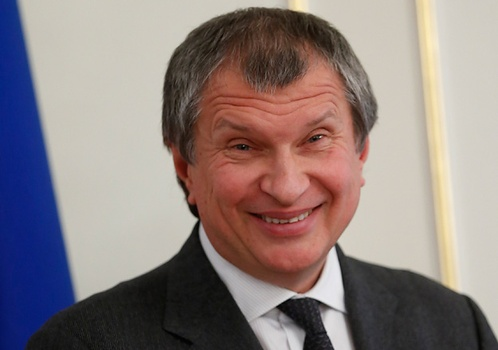
\includegraphics[scale=0.6]{sechin1.jpg}
 \end{center}
Ладно-ладно, вот \\
\begin{center}

\includegraphics[scale=0.5]{Durov.jpg}
\end{center}

\section{Формулы}
Вот любимые:

\begin{equation}\label{eq1}
\Gamma (z) = \int_{0}^{+\infty} t^{z-1} \cdot e^{-t} dt  \tag{\ae}
\end{equation}

\begin{equation}\label{eq2}
\Gamma (z) =  \lim\limits_{n\to\infty} \frac{(n-1)!n^z}{z(z+1)(z+2)\cdots(z+n-1)} \qquad z \in \C \setminus \{0,-1,-2, \dots \} \tag{\ae\ae}
\end{equation}

\begin{equation}\label{eq3}
\hat{\beta} = \frac{\sum_{i=1}^{n}(x_i-\bar{x})y_i}{\sum_{i=1}^{n}(x_i-\bar{x})^2}  \tag{\ae\ae\ae}
\end{equation}
\begin{equation}\label{eq4}
 \begin{pmatrix}
y_1 \\
\vdots \\
y_n
 \end{pmatrix} =
 \begin{pmatrix}
 1 & x_{1,1} &\cdots & x_{k,1}\\
 && \ddots & \\
 1 & x_{1,n} &\cdots & x_{k,n}
 \end{pmatrix}
 \begin{pmatrix}
 \beta_0 \\
 \vdots \\
 \beta_k
 \end{pmatrix} \tag{\ae\ae\ae\ae}
\end{equation}

\label{eq5}
  \begin{align}
\hat{u_i} &=\delta_0+\delta_1 z_{1,i} + \delta_2 z_{2,i}+ \ldots + \delta_r z_{r,i}+ \\
& \delta_{r+1} w_{1,i} + \delta_{r+2} w_{2,i} + \ldots + \delta_{r+m} w_{m,i} +\varepsilon_i  \label{eq5}
 \tag{\ae\ae\ae\ae\ae}
  \end{align} 


А теперь посложнее:\\
\begin{equation}\label{eq6}
\widehat {Var(\hat{\beta_1})} = \frac{1}{n} \cdot \frac{ \frac{1}{n-2}  \sum_{i=1}^{n} (x_i-\bar{x})^2 \hat{u_i}^2} { [\frac{1}{n} \sum_{i=1}^{n}(x_i-\bar{x})^2]^2} \tag{\ae\ae\ae\ae\ae\ae}
\end{equation}

Формула \eqref{eq1} --- гамма-функция Эйлера, которая используется при расчете характеристик многих статистических распределений, а формула \eqref{eq2} --- гамма-функций по Гауссу. Формула \eqref{eq3} --- знакомое всем выражение оценки $\beta_1$ в модели парной линейной регрессии. Выражение \eqref{eq4} представляет собой матричную запись модели множественной регрессии, а \eqeref{eq5} --- модель для тестирования сверхидентифицирующих ограничений в TSLS. У выражения \eqref{eq6}даже в названии можно запутаться --- это формула оценки диспресии оценки коэффициента $\beta_1$ в модели парной регресси. Для $\beta_0$ кстати противнее. 

\end{document}	